\documentclass[12pt]{article}
\usepackage{amsmath, amssymb}
\usepackage{hyperref}
\usepackage{graphicx}
\usepackage{tikz}
\setlength{\parindent}{0pt}

\title{Probearbeit 2}
\author{}
\date{04.12.2025}

\begin{document}
\maketitle

\textbf{Hinweis.} Begründe alle Schritte. Achte besonders auf Vorzeichen (Doppelminus!) und auf sauberes Arbeiten mit Brüchen. Exakte Werte sind ausreichend. Skizzen müssen nicht maßstäblich sein, aber wichtige Punkte sollen beschriftet werden.

\section*{Aufgabe 1: Punkte berechnen und skizzieren}
Betrachte \(f(x) = -\tfrac{1}{2}(x-1)^{2} + \tfrac{7}{2}\).
\begin{enumerate}
  \item Berechne \(f(x)\) für \(x = -1, 0, 1, 2, 3\) und trage die Werte in die Tabelle ein.
  \item Gib Scheitelpunkt, Symmetrieachse und Öffnungsrichtung an.
  \item Zeichne die Parabel mithilfe der berechneten Punkte. Trage Scheitelpunkt und Symmetrieachse im Koordinatensystem unten ein.
\end{enumerate}

\begin{center}
\begingroup
\renewcommand{\arraystretch}{1.8}
\begin{tabular}{|c|c|c|c|c|c|}
  \hline
  \(x\) & \(-1\) & \(0\) & \(1\) & \(2\) & \(3\) \\
  \hline
  \(y = f(x)\) & & & & & \\
  \hline
\end{tabular}
\endgroup
\end{center}

\begin{center}
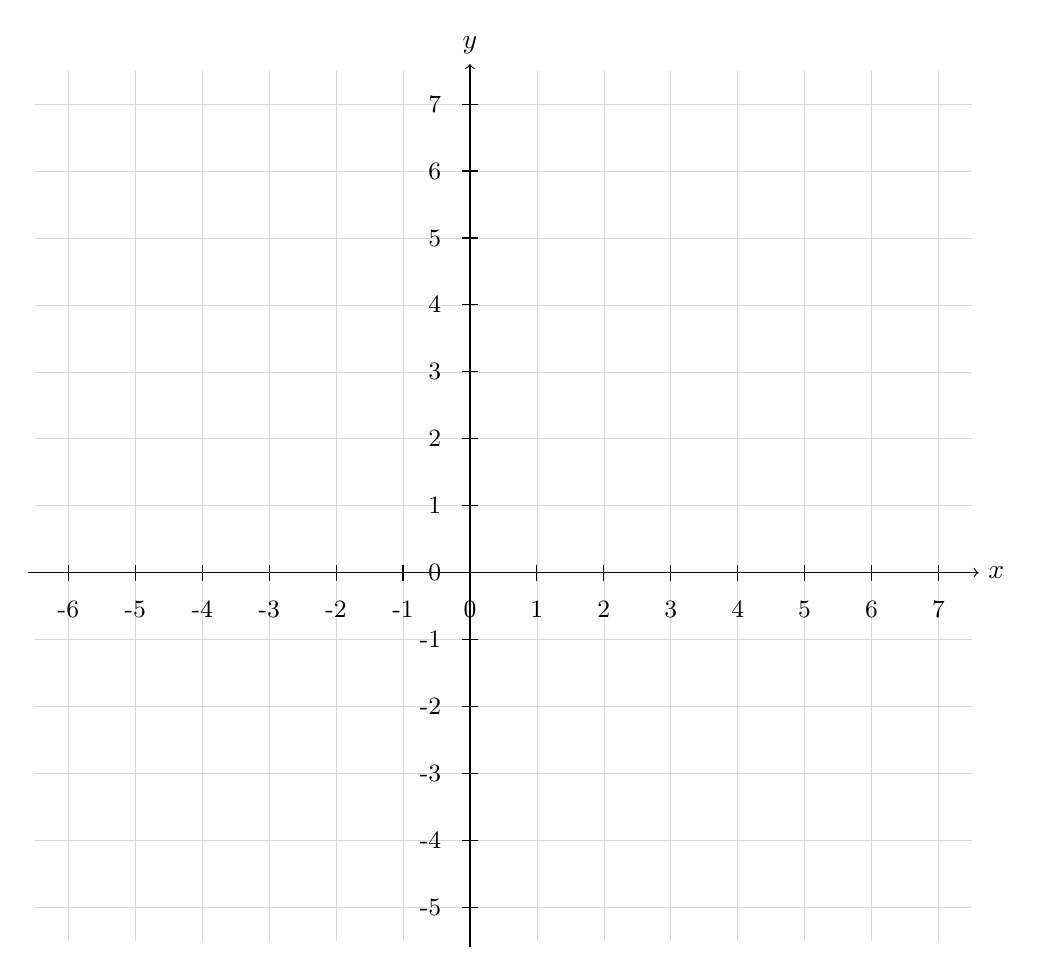
\begin{tikzpicture}[scale=0.85]
  \draw[step=1cm,gray!30,very thin] (-6.5,-5.5) grid (7.5,7.5);
  \draw[->] (-6.6,0) -- (7.6,0) node[right] {$x$};
  \draw[->] (0,-5.6) -- (0,7.6) node[above] {$y$};
  \foreach \x in {-6,-5,...,7} \draw (\x,0.12) -- (\x,-0.12) node[below=4pt] {\small \x};
  \foreach \y in {-5,-4,...,7} \draw (0.12,\y) -- (-0.12,\y) node[left=4pt] {\small \y};
\end{tikzpicture}
\end{center}

\section*{Aufgabe 2: Nullstellen mit der PQ-Formel}
Die PQ-Formel für \(x^{2} + px + q = 0\) lautet
\[
  x_{1,2} = -\frac{p}{2} \pm \sqrt{\left(\frac{p}{2}\right)^{2} - q}.
\]
Bestimme damit die \(x\)-Achsenabschnitte der Parabel \(y = x^{2} + 3x - 10\). Nenne beide Nullstellen und gib an, ob die Parabel die \(x\)-Achse dort schneidet oder berührt.

\section*{Aufgabe 3: Skizze aus Scheitelpunktform}
Skizziere den Graphen von \(g(x) = -\tfrac{2}{3}(x+1)^{2} + 5\) im Koordinatensystem. Beschrifte Scheitelpunkt, \(y\)-Achsenabschnitt und vorhandene \(x\)-Achsenabschnitte.

\begin{center}
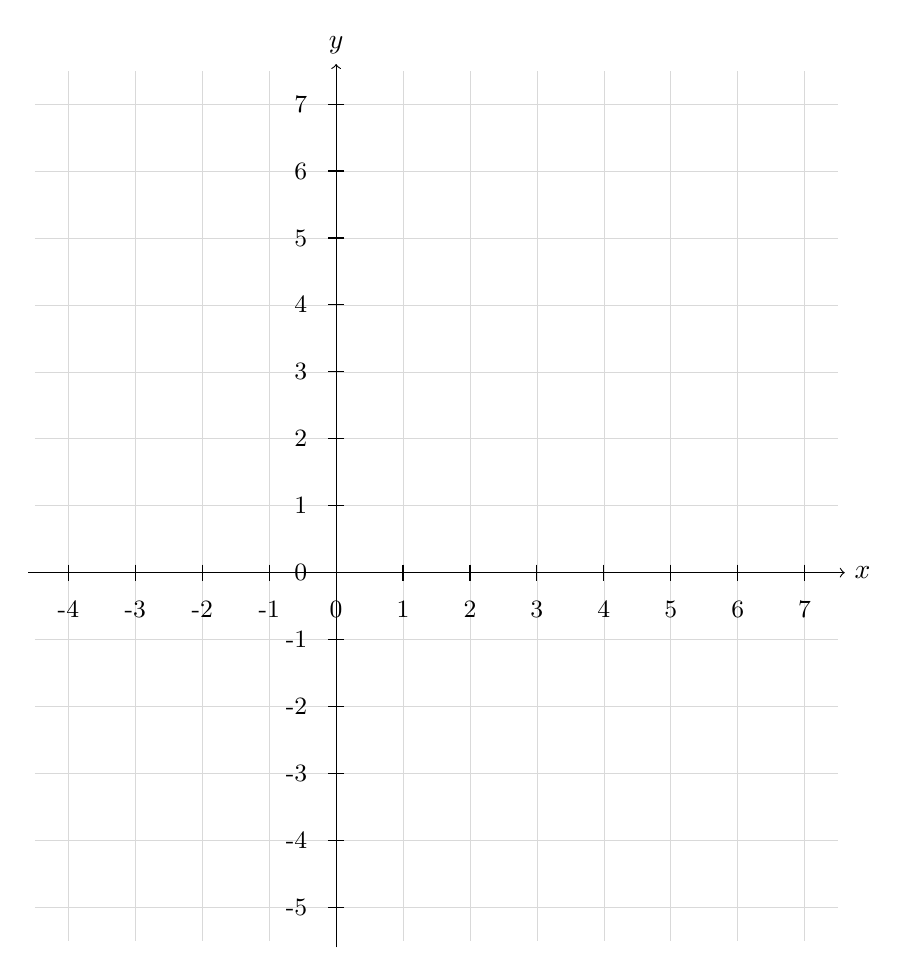
\begin{tikzpicture}[scale=0.85]
  \draw[step=1cm,gray!30,very thin] (-4.5,-5.5) grid (7.5,7.5);
  \draw[->] (-4.6,0) -- (7.6,0) node[right] {$x$};
  \draw[->] (0,-5.6) -- (0,7.6) node[above] {$y$};
  \foreach \x in {-4,-3,...,7} \draw (\x,0.12) -- (\x,-0.12) node[below=4pt] {\small \x};
  \foreach \y in {-5,-4,...,7} \draw (0.12,\y) -- (-0.12,\y) node[left=4pt] {\small \y};
\end{tikzpicture}
\end{center}

\newpage
\section*{Aufgabe 4: Tiefpunkt und Eigenschaften einer nach oben offenen Parabel}
Für \(h(x) = \tfrac{1}{4}x^{2} + x - 3\):
\begin{enumerate}
  \item Schreibe \(h(x)\) in Scheitelpunktform (achte auf Doppelminus beim Ausklammern).
  \item Bestimme den Tiefpunkt (Koordinaten) und den minimalen Funktionswert.
  \item Gib die Gleichung der Symmetrieachse an.
  \item Berechne die Nullstellen (falls vorhanden) mit der PQ-Formel. Notiere, ob die Parabel die \(x\)-Achse schneidet oder berührt.
  \item Bestimme den \(y\)-Achsenabschnitt.
  \item Skizziere \(h\) und markiere Scheitelpunkt, Achsenschnittpunkte und Symmetrieachse. Nutze bei Bedarf zwei zusätzliche Punkte deiner Wahl.
\end{enumerate}

\end{document}
